%%%%%%%%%%%%%%%%%%%%%%%%%%%%%%%%%%%%%%%%%
% Beamer Presentation
% LaTeX Template
% Version 2.0 (March 8, 2022)
%
% This template originates from:
% https://www.LaTeXTemplates.com
%
% Author:
% Vel (vel@latextemplates.com)
%
% License:
% CC BY-NC-SA 4.0 (https://creativecommons.org/licenses/by-nc-sa/4.0/)
%
%%%%%%%%%%%%%%%%%%%%%%%%%%%%%%%%%%%%%%%%%

%----------------------------------------------------------------------------------------
%	PACKAGES AND OTHER DOCUMENT CONFIGURATIONS
%----------------------------------------------------------------------------------------
\documentclass[
  24pt, % Set the default font size, options include: 8pt, 9pt, 10pt, 11pt, 12pt, 14pt, 17pt, 20pt
  %t, % Uncomment to vertically align all slide content to the top of the slide, rather than the default centered
  aspectratio=169, % Uncomment to set the aspect ratio to a 16:9 ratio which matches the aspect ratio of 1080p and 4K screens and projectors
]{beamer}

\graphicspath{{Images/}{./}} % Specifies where to look for included images (trailing slash required)

\usepackage{booktabs} % Allows the use of \toprule, \midrule and \bottomrule for better rules in tables

%----------------------------------------------------------------------------------------
%	SELECT LAYOUT THEME
%----------------------------------------------------------------------------------------

% Beamer comes with a number of default layout themes which change the colors and layouts of slides. Below is a list of all themes available, uncomment each in turn to see what they look like.

%\usetheme{default}
%\usetheme{AnnArbor}
%\usetheme{Antibes}
%\usetheme{Bergen}
%\usetheme{Berkeley}
%\usetheme{Berlin}
\usetheme{Boadilla} %me gusta
%\usetheme{CambridgeUS}
%\usetheme{Copenhagen}
%\usetheme{Darmstadt}
%\usetheme{Dresden}
%\usetheme{Frankfurt}
%\usetheme{Goettingen} %dos dos
%\usetheme{Hannover} %dos dos
%\usetheme{Ilmenau}
%\usetheme{JuanLesPins}
%\usetheme{Luebeck}
%\usetheme{Madrid}
%\usetheme{Malmoe}
%\usetheme{Marburg}
%\usetheme{Montpellier}
%\usetheme{PaloAlto}
%\usetheme{Pittsburgh}
%\usetheme{Rochester} %muy flat
%\usetheme{Singapore}
%\usetheme{Szeged}
%\usetheme{Warsaw}

%----------------------------------------------------------------------------------------
%	SELECT COLOR THEME
%----------------------------------------------------------------------------------------

% Beamer comes with a number of color themes that can be applied to any layout theme to change its colors. Uncomment each of these in turn to see how they change the colors of your selected layout theme.

%\usecolortheme{albatross}
%\usecolortheme{beaver}
%\usecolortheme{beetle}
%\usecolortheme{crane}
%\usecolortheme{dolphin}
%\usecolortheme{dove}
%\usecolortheme{fly}
%\usecolortheme{lily} %default
%\usecolortheme{monarca}
%\usecolortheme{seagull}
%\usecolortheme{seahorse}
%\usecolortheme{spruce}
%\usecolortheme{whale}
%\usecolortheme{wolverine}

%----------------------------------------------------------------------------------------
%	SELECT FONT THEME & FONTS
%----------------------------------------------------------------------------------------

% Beamer comes with several font themes to easily change the fonts used in various parts of the presentation. Review the comments beside each one to decide if you would like to use it. Note that additional options can be specified for several of these font themes, consult the beamer documentation for more information.

\usefonttheme{default} % Typeset using the default sans serif font
%\usefonttheme{serif} % Typeset using the default serif font (make sure a sans font isn't being set as the default font if you use this option!)
%\usefonttheme{structurebold} % Typeset important structure text (titles, headlines, footlines, sidebar, etc) in bold
%\usefonttheme{structureitalicserif} % Typeset important structure text (titles, headlines, footlines, sidebar, etc) in italic serif
%\usefonttheme{structuresmallcapsserif} % Typeset important structure text (titles, headlines, footlines, sidebar, etc) in small caps serif

%------------------------------------------------

%\usepackage{mathptmx} % Use the Times font for serif text
\usepackage{palatino} % Use the Palatino font for serif text

\usepackage[ruled,vlined]{algorithm2e}
%\usepackage{helvet} % Use the Helvetica font for sans serif text
\usepackage[default]{opensans} % Use the Open Sans font for sans serif text
\usepackage[spanish]{babel}
\usepackage{dirtree}
\usepackage{xcolor}
%\usepackage[default]{FiraSans} % Use the Fira Sans font for sans serif text
%\usepackage[default]{lato} % Use the Lato font for sans serif text

\usepackage[scaled]{helvet}
\usepackage[round]{natbib}
%\newcommand{\newblock}{}

\usepackage{rotating}

\newcommand\FourQuad[4]{%
  \begin{minipage}[b][.33\textheight][t] 
    {.48\textwidth}#1\end{minipage}\hfill%
    \begin{minipage}[b][.33\textheight][t] 
      {.48\textwidth}#2\end{minipage}\\[0.5em]
      \begin{minipage}[b][.33\textheight][t] 
        {.48\textwidth}#3\end{minipage}\hfill
        \begin{minipage}[b][.33\textheight][t] 
          {.48\textwidth}#4\end{minipage}%
}

\usepackage{tikz}
%\usetikzlibrary{arrows,shapes,positioning,shadows,trees,quotes}


%\tikzset{
%  basic/.style  = {draw, text width=2cm, drop shadow, font=\sffamily, rectangle},
%  root/.style   = {basic, rounded corners=2pt, thin, align=center,
%                   fill=green!30},
%  level 2/.style = {basic, rounded corners=6pt, thin,align=center, fill=green!60,
%                   text width=8em},
%  level 3/.style = {basic, thin, align=left, fill=pink!60, text width=6.5em}
%}

\usetikzlibrary{calc}

\tikzstyle{part} = [rectangle, rounded corners, minimum width=3cm, minimum height=1cm,     align=center, draw=black]
\tikzstyle{chapter} = [rectangle, rounded corners, minimum width=3cm, minimum height=1cm,     align=center, draw=black, text width=3.5cm]
\tikzstyle{arrow} = [thick, ->]

\usepackage{array} % needed for \arraybackslash
\usepackage{graphicx}
\usepackage{adjustbox} % for \adjincludegraphics

\usepackage{subcaption}
\usepackage{bibentry}
%\bibliographystyle{apalike}
\usepackage{chngcntr}
\usepackage{lipsum}% http://ctan.org/pkg/lipsum
\usepackage{hanging}% http://ctan.org/pkg/hanging

\usepackage{xcolor,colortbl}
\usepackage{multirow}

\usepackage{animate}
\usepackage{multicol}
\usepackage{tabularx,booktabs}
\usepackage{forloop}
\usepackage{ragged2e}

\usepackage{bbding} %palomitas checkmark
\usepackage{pifont}
\usepackage{lipsum,tabularx}

\newcounter{loopcntr}

%----------------------------------------------------------------------------------------
%	SELECT INNER THEME
%----------------------------------------------------------------------------------------

% Inner themes change the styling of internal slide elements, for example: bullet points, blocks, bibliography entries, title pages, theorems, etc. Uncomment each theme in turn to see what changes it makes to your presentation.

\useinnertheme{circles}

%----------------------------------------------------------------------------------------
%	SELECT OUTER THEME
%----------------------------------------------------------------------------------------

% Outer themes change the overall layout of slides, such as: header and footer lines, sidebars and slide titles. Uncomment each theme in turn to see what changes it makes to your presentation.

\setbeamertemplate{footline}[frame number] % Uncomment this line to replace the footer line in all slides with a simple slide count
\setbeamertemplate{navigation symbols}{} % Uncomment this line to remove the navigation symbols from the bottom of all slides

%----------------------------------------------------------------------------------------
%	PRESENTATION INFORMATION
%----------------------------------------------------------------------------------------

\title[PRESENTACION 4]{%\centering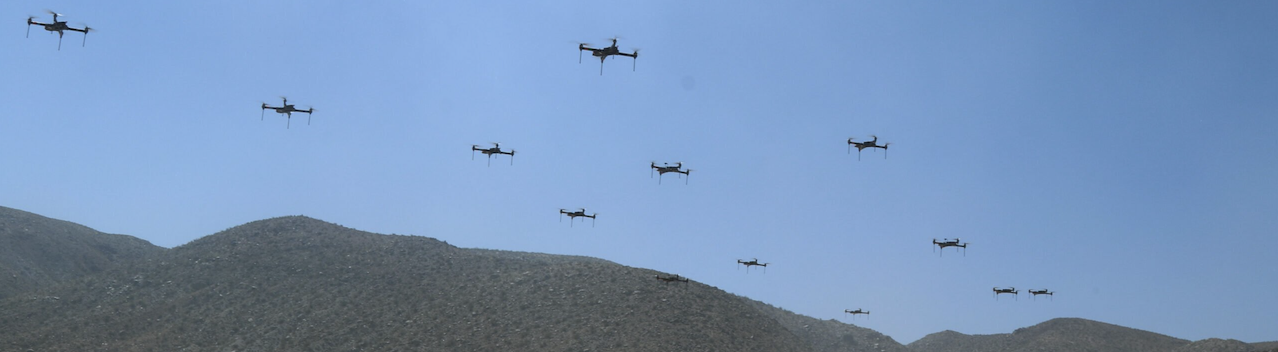
\includegraphics[width=10cm]{swarm_drones}\\
  Estrategias para la exploración coordinada multi-VANT} % The short title in the optional parameter appears at the bottom of every slide, the full title in the main parameter is only on the title page

%\subtitle{Optional Subtitle} % Presentation subtitle, remove this command if a subtitle isn't required

\author[]{Luis Alberto Ballado Aradias\\[\baselineskip]
  \small{{Asesores:} \\
    \and\\Dr. José Gabriel Ramírez-Torres
    \and\\Dr. Eduardo Rodriguez-Tello }}

\institute[CINVESTAV]{
  CINVESTAV UNIDAD TAMAULIPAS \\
  %\smallskip \textit{luis.ballado@cinvestav.mx}
} % Your institution, the optional parameter can be used for the institution shorthand and will appear on the bottom of every slide after author names, while the required parameter is used on the title slide and can include your email address or additional information on separate lines


\date[\today]{Cd. Victoria, Tamaulipas - 16 Abril 2024} % Presentation date or conference/meeting name, the optional parameter can contain a shortened version to appear on the bottom of every slide, while the required parameter value is output to the title slide

%\titlegraphic{\hspace*{8.75cm}~%
%   
\includegraphics[width=0.8cm]{cinvestavlogo}
%}

%----------------------------------------------------------------------------------------

\counterwithin*{footnote}{page}
\newcommand\footcite[1]{\footnote{\bibentry{#1}}\label{\thepage:#1}}
\newcommand\secondcite[1]{\textsuperscript{\ref{\thepage:#1}}}

\newcommand{\rpt}[2][1]{%
  \forloop{loopcntr}{0}{\value{loopcntr}<#1}{#2}%
}
\newcommand{\on}[1][1]{
  \forloop{loopcntr}{0}{\value{loopcntr}<#1}{&\cellcolor{gray}}
}
\newcommand{\onok}[1][1]{
  \forloop{loopcntr}{0}{\value{loopcntr}<#1}{&\cellcolor{green}}
}
\newcommand{\off}[1][1]{
  \forloop{loopcntr}{0}{\value{loopcntr}<#1}{&\cellcolor{white}}
}

\addtolength{\textheight}{90pt}

\newcommand{\I}{\mathbb{I}}
\newcommand{\K}{\mathbb{K}}
\newcommand{\N}{\mathbb{N}}
\newcommand{\Q}{\mathbb{Q}}
\newcommand{\R}{\mathbb{R}}
\newcommand{\Z}{\mathbb{Z}}

\newcommand{\specialcell}[2][c]{%
  \begin{tabular}[#1]{@{}c@{}}#2\end{tabular}}


\begin{document}

%----------------------------------------------------------------------------------------
%	TITLE SLIDE
%----------------------------------------------------------------------------------------

\begin{frame}
  \titlepage % Output the title slide, automatically created using the text entered in the PRESENTATION INFORMATION block above
\end{frame}

%----------------------------------------------------------------------------------------
%	TABLE OF CONTENTS SLIDE
%----------------------------------------------------------------------------------------

% The table of contents outputs the sections and subsections that appear in your presentation, specified with the standard \section and \subsection commands. You may either display all sections and subsections on one slide with \tableofcontents, or display each section at a time on subsequent slides with \tableofcontents[pausesections]. The latter is useful if you want to step through each section and mention what you will discuss.
\AtBeginSection[]
{
  \begin{frame}
    \frametitle{Contenido} % Slide title, remove this command for no title
    \tableofcontents[currentsection] % Output the table of contents (all sections on one slide)
    %\tableofcontents[pausesections] % Output the table of contents (break sections up across separate slides)
  \end{frame}
}

\pretocmd{\tableofcontents}{\thispagestyle{empty}}{}{}

%----------------------------------------------------------------------------------------
%	PRESENTATION BODY SLIDES
%----------------------------------------------------------------------------------------

\section{Antecedentes y motivación del proyecto}
\begin{frame}{Antecedentes}
  \bigskip % Vertical whitespace
  \centering
  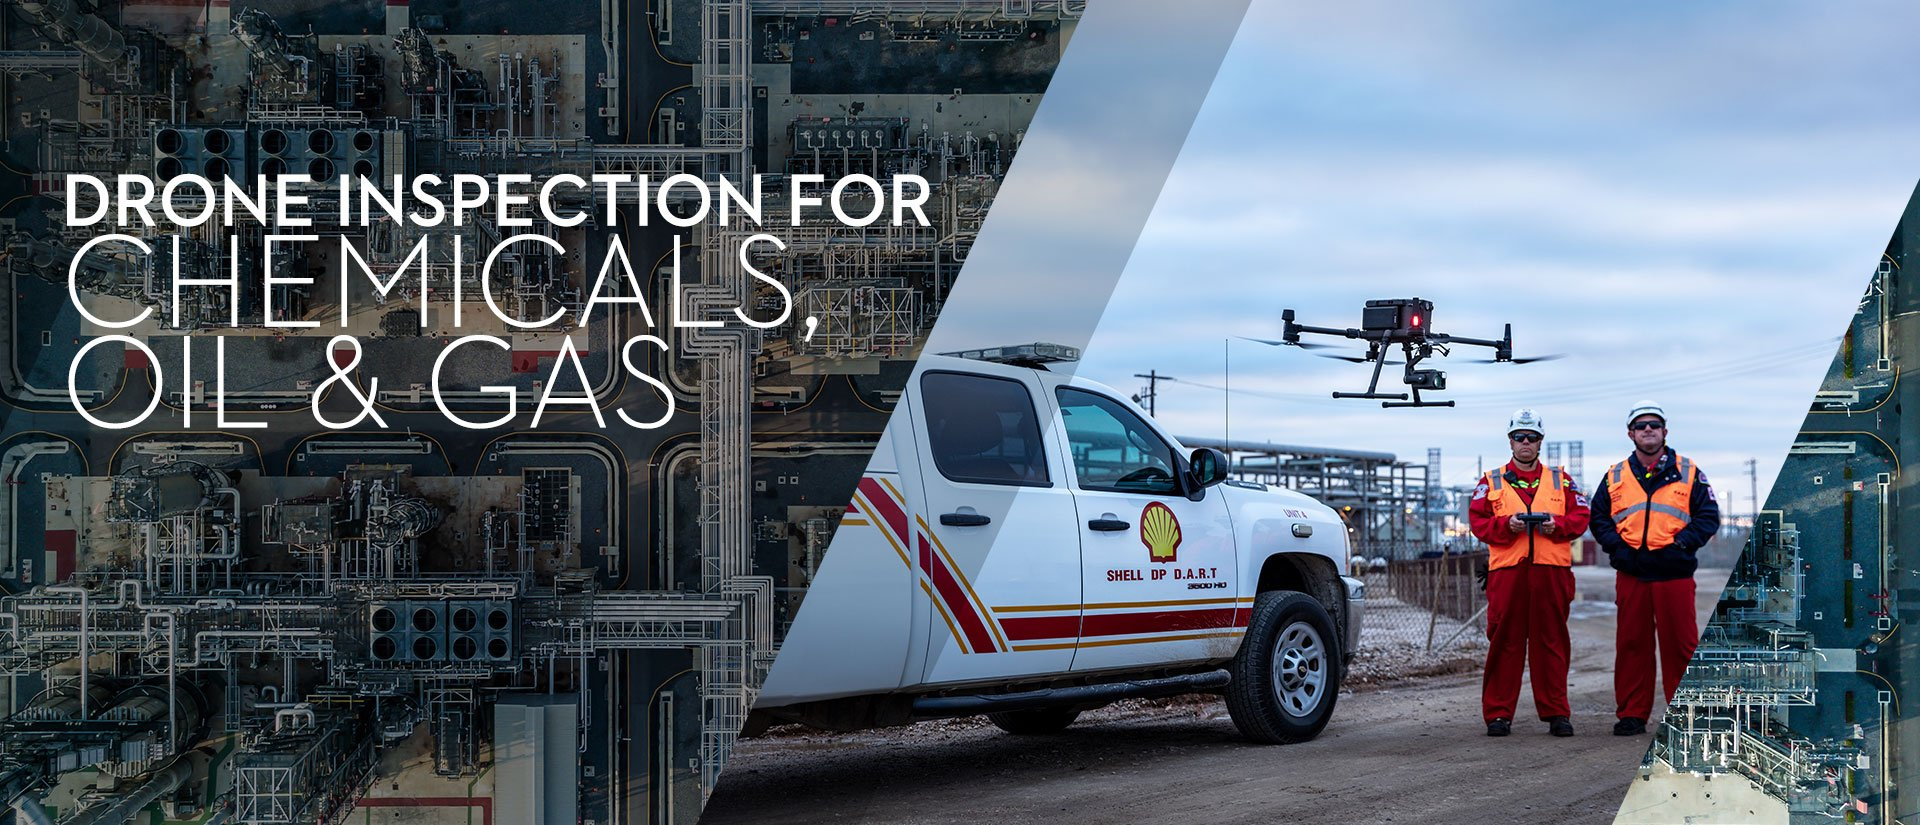
\includegraphics[width=0.45\textwidth,height=0.35\textheight]{DJI_B4}
  \hfil
  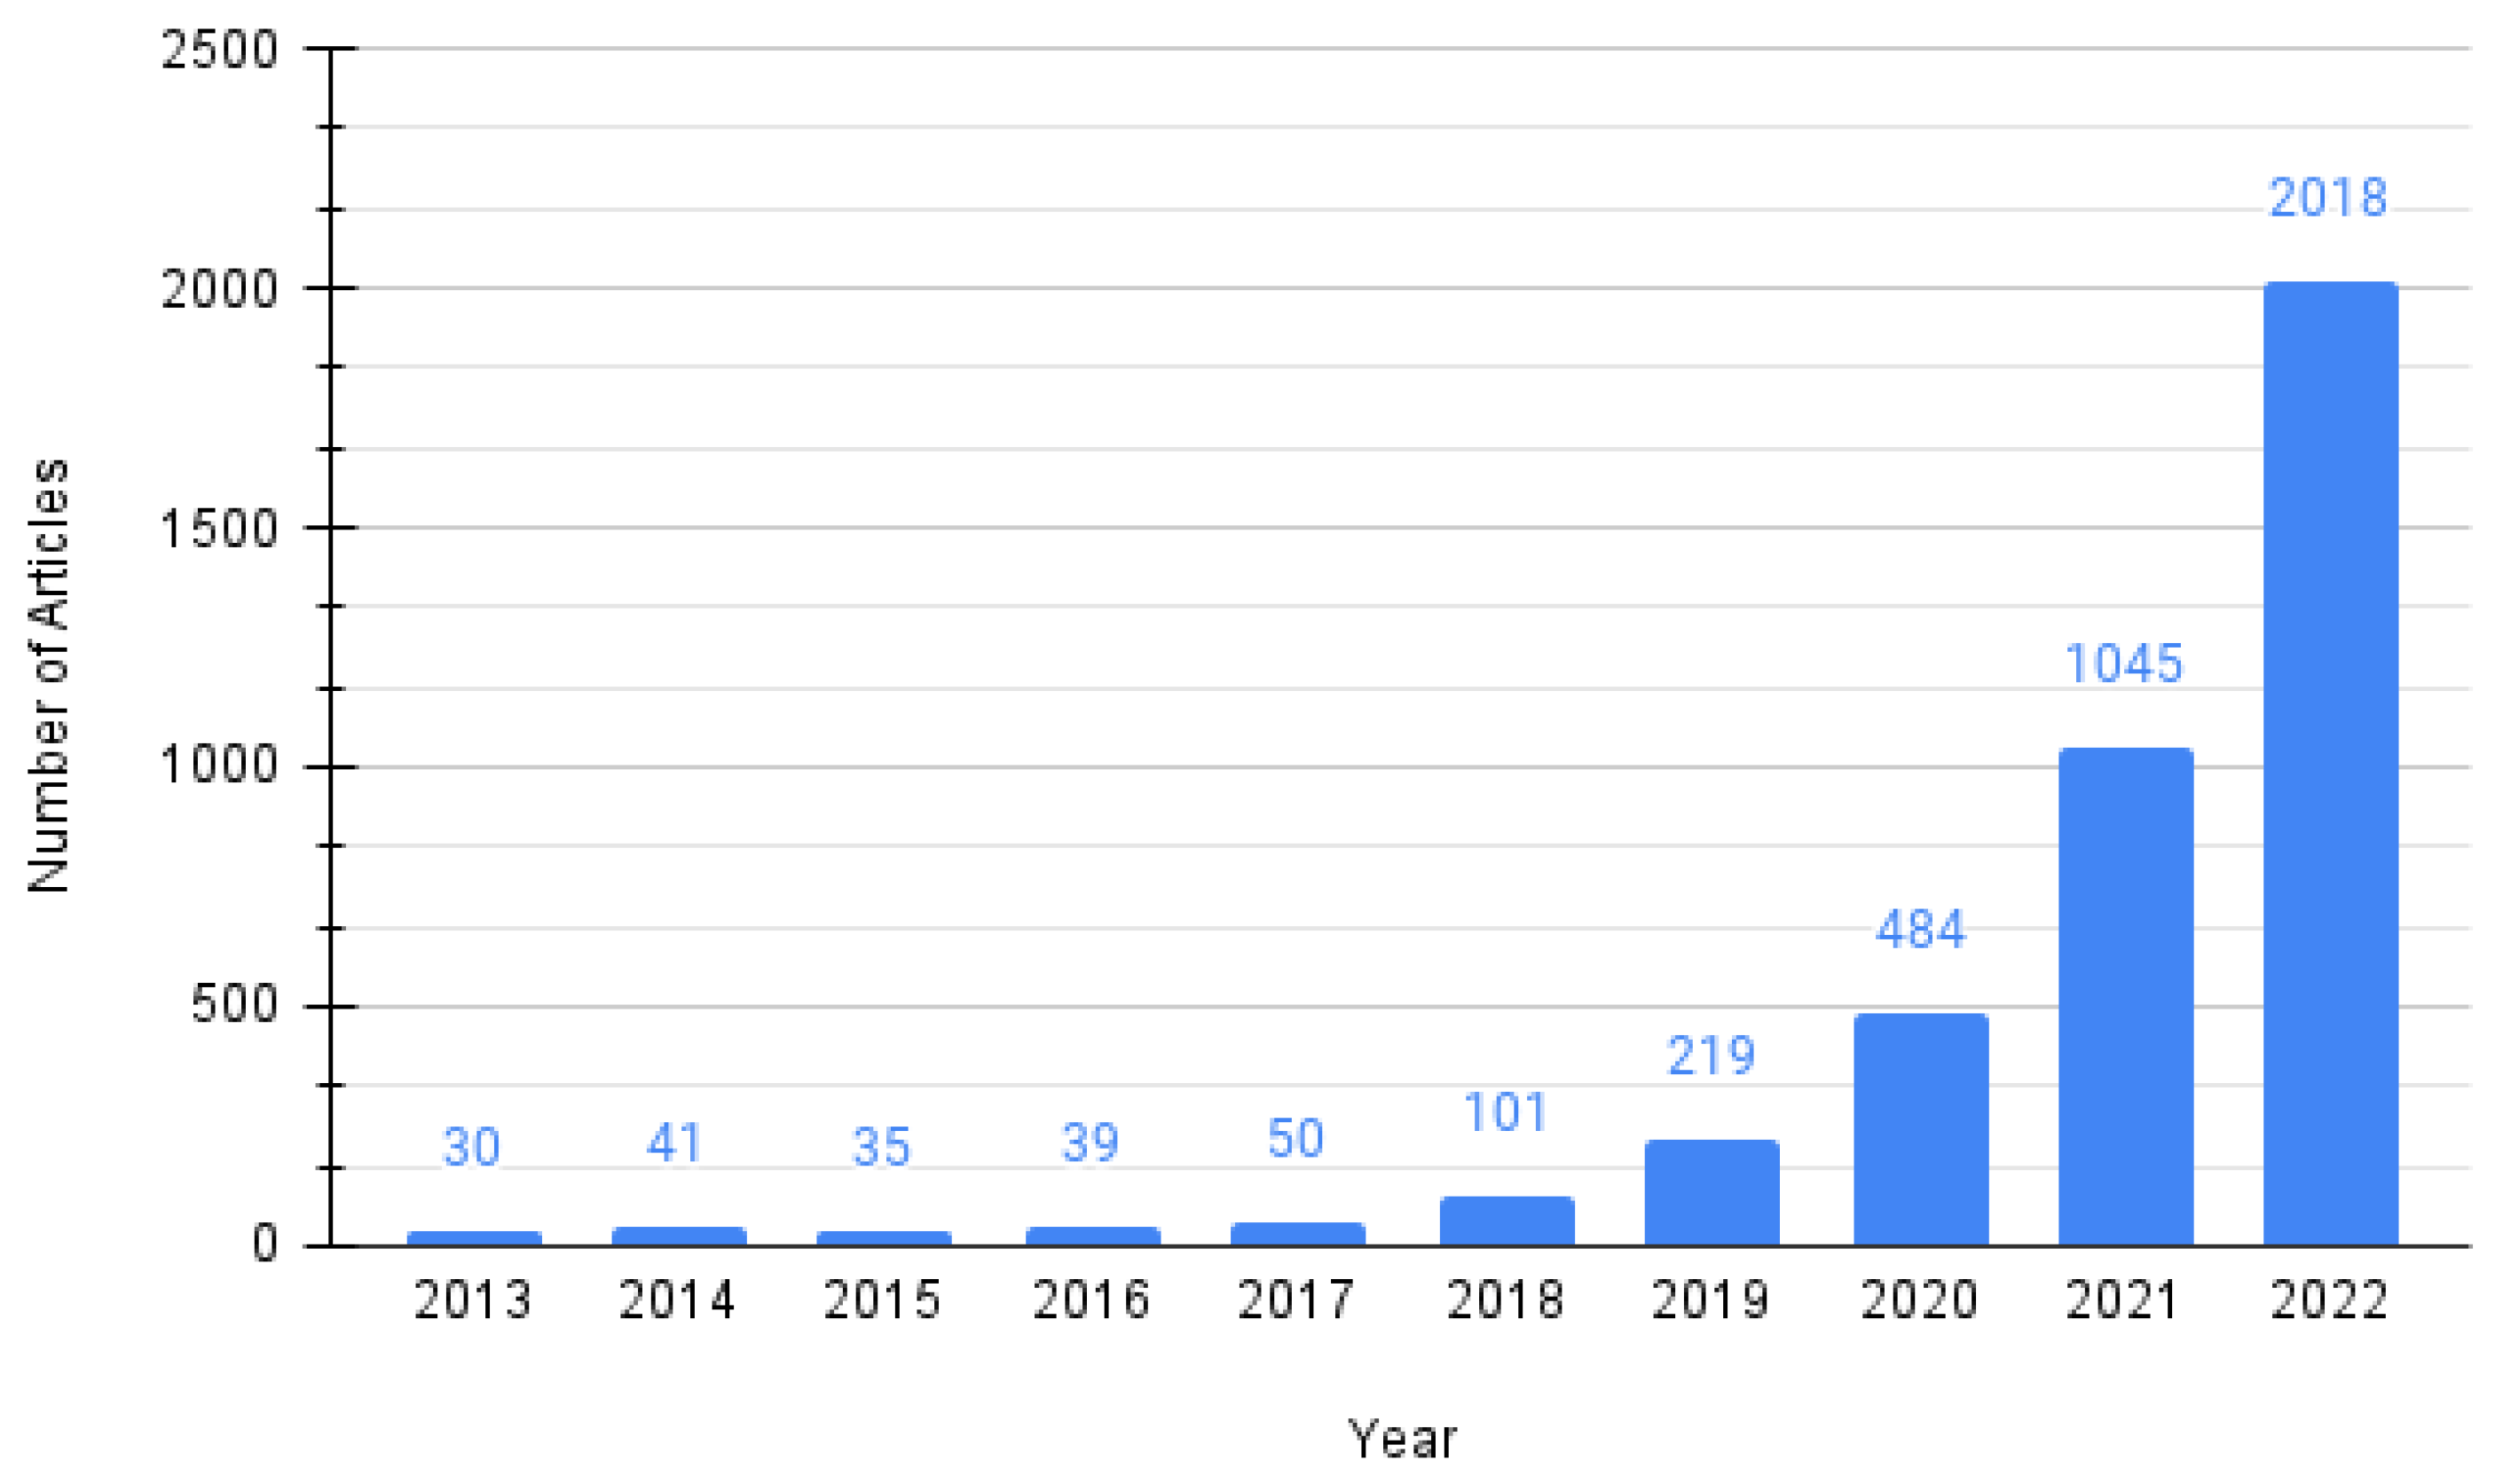
\includegraphics[width=0.45\textwidth,height=0.35\textheight]{drones-07-00236-g001.png}\footnotemark
  \vspace{2pt}\\
  
  \begin{itemize}
  \item \textbf{UAV} {\tiny(\textit{Vehículo Aéreo No Tripulado - VANT})}  $\implies$ \textbf{UAS} {\tiny(\textit{Sistemas Aéreos No Tripulado - SANT})}
  \item \textbf{Aplicaciones} en lugares inaccesibles o peligrosos.
  \item \textbf{Múltiples VANT} pueden reducir el tiempo de exploración y aumentar la confianza del sistema.
  \item \textbf{Limitaciones} en carga, procesamiento y batería influyen en el tiempo de vuelo.
  \end{itemize}
  
  \footnotetext{UAV in the advent of the twenties: Where we stand and what is next [\cite{Nex2022}]}
  %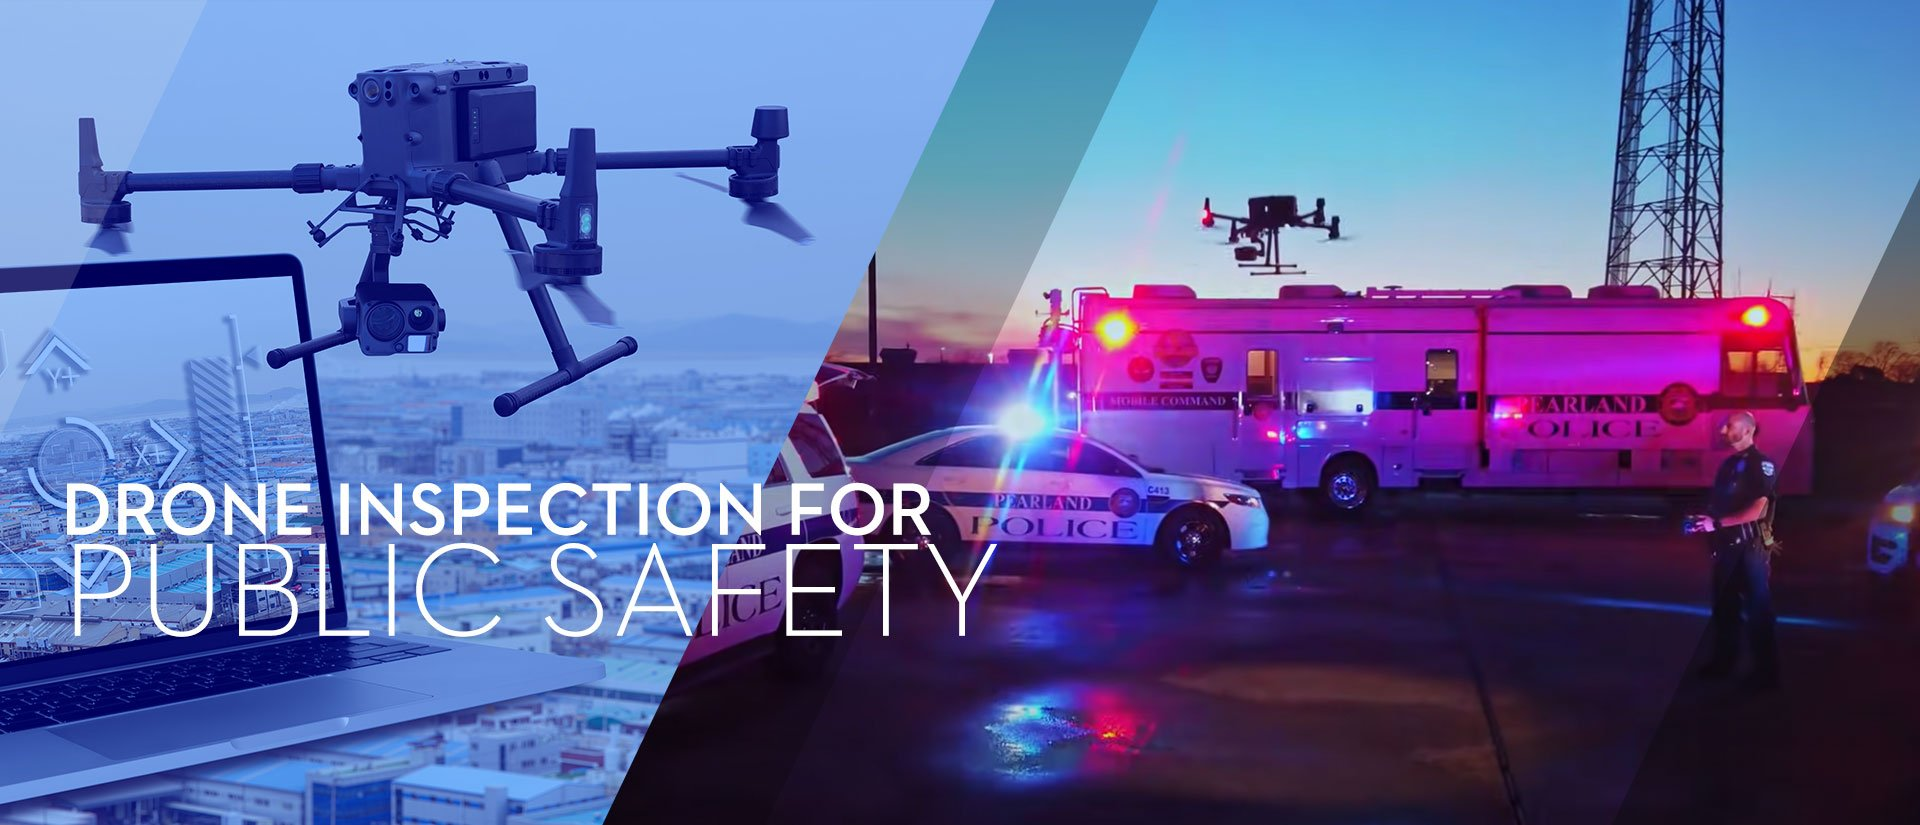
\includegraphics[width=0.45\textwidth,height=0.35\textheight]{DJI_B5}$^\dag$ 
  %\hfil
  %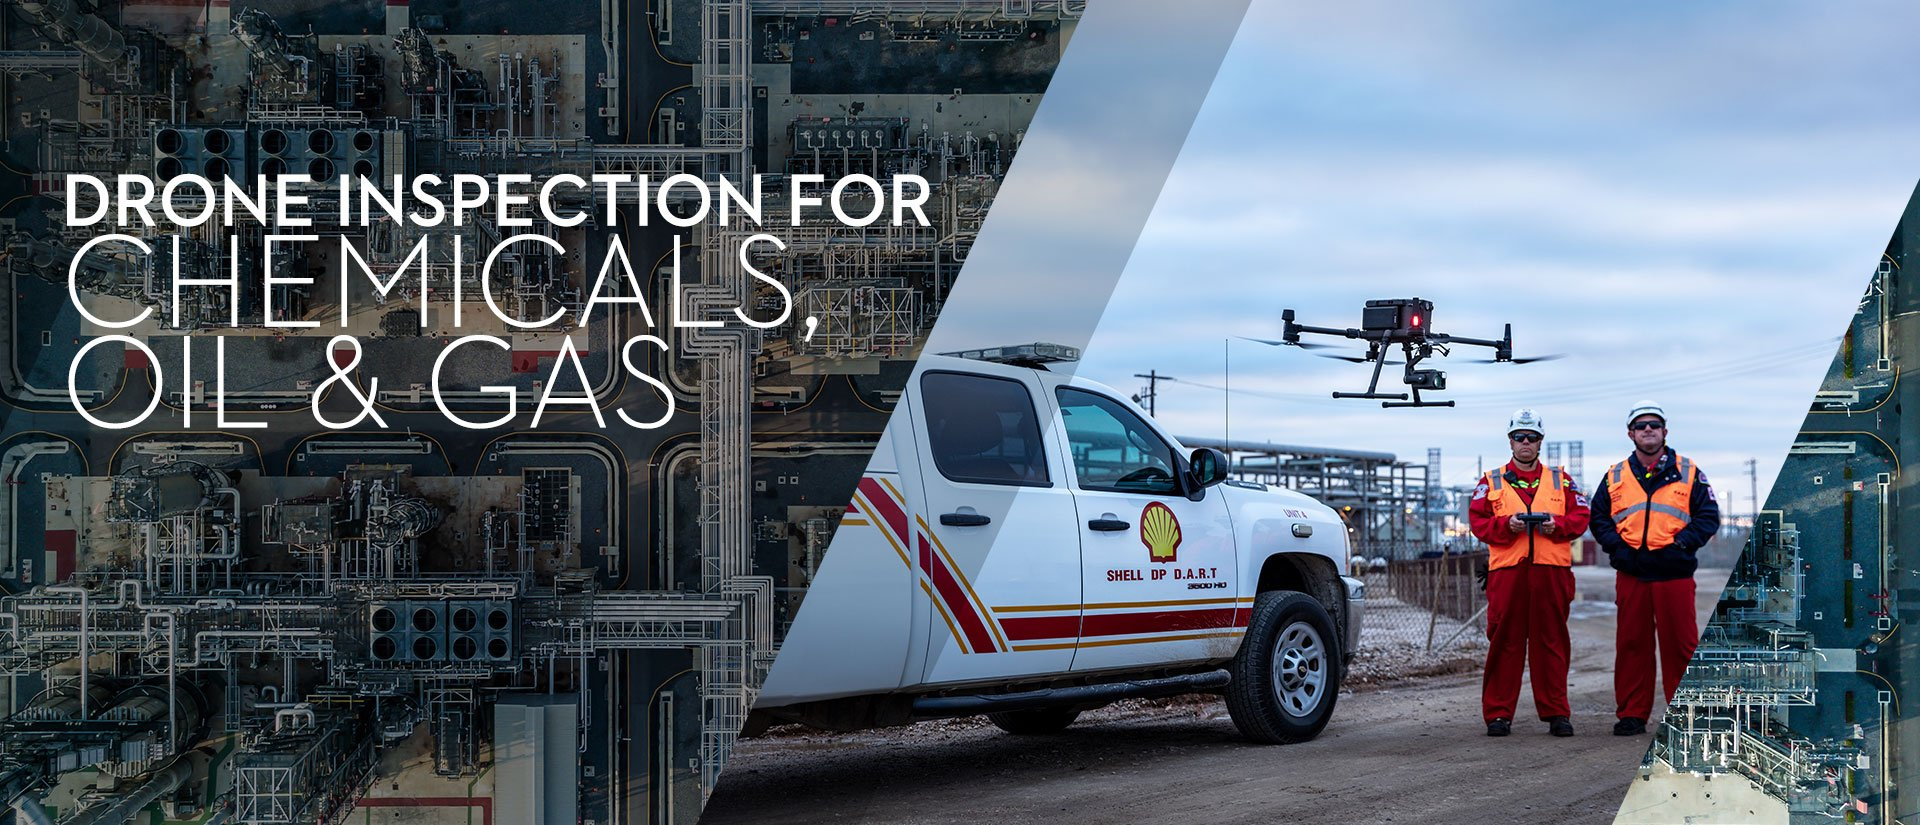
\includegraphics[width=0.45\textwidth,height=0.35\textheight]{DJI_B4}$^\dag$\\
  %\rule{0in}{1.2em}$^\dag$ \small Inspecciones con VANT basadas en los mejores casos de uso\\
  %\tiny \url{https://enterprise-insights.dji.com/blog/complete-guide-to-drone-inspections}
\end{frame}

\begin{frame}{Motivación del proyecto}
  %https://ccc.inaoep.mx/~emorales/Papers/2009/eduardo.pdf
  %https://www.mdpi.com/2504-446X/7/1/62
  Hablar de los usos e importancia del trabajo .. de la exploracion .. de la importancia de investigacion en robotica para el pais.
  \begin{figure}[ht!]
        \centering
        \begin{minipage}{0.48\textwidth}
            \centering
            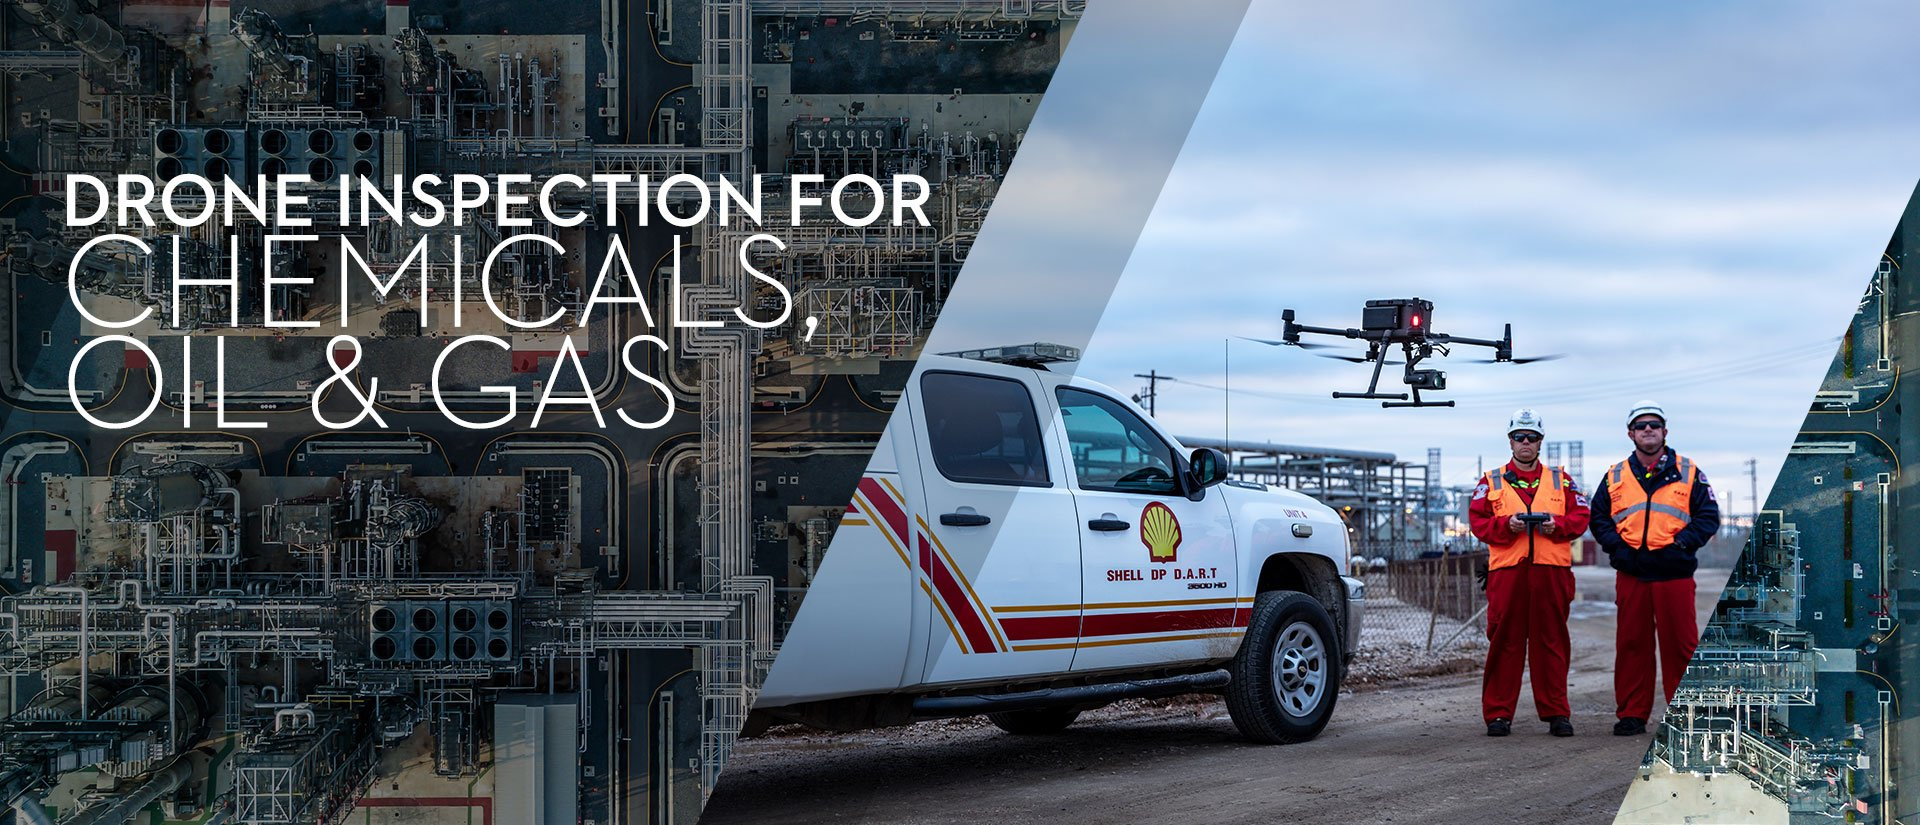
\includegraphics[width=\linewidth]{DJI_B4} % Reemplazar con la ruta a tu imagen
            %\caption{Primera Imagen}
        \end{minipage}\hfill
        \begin{minipage}{0.48\textwidth}
            \centering
            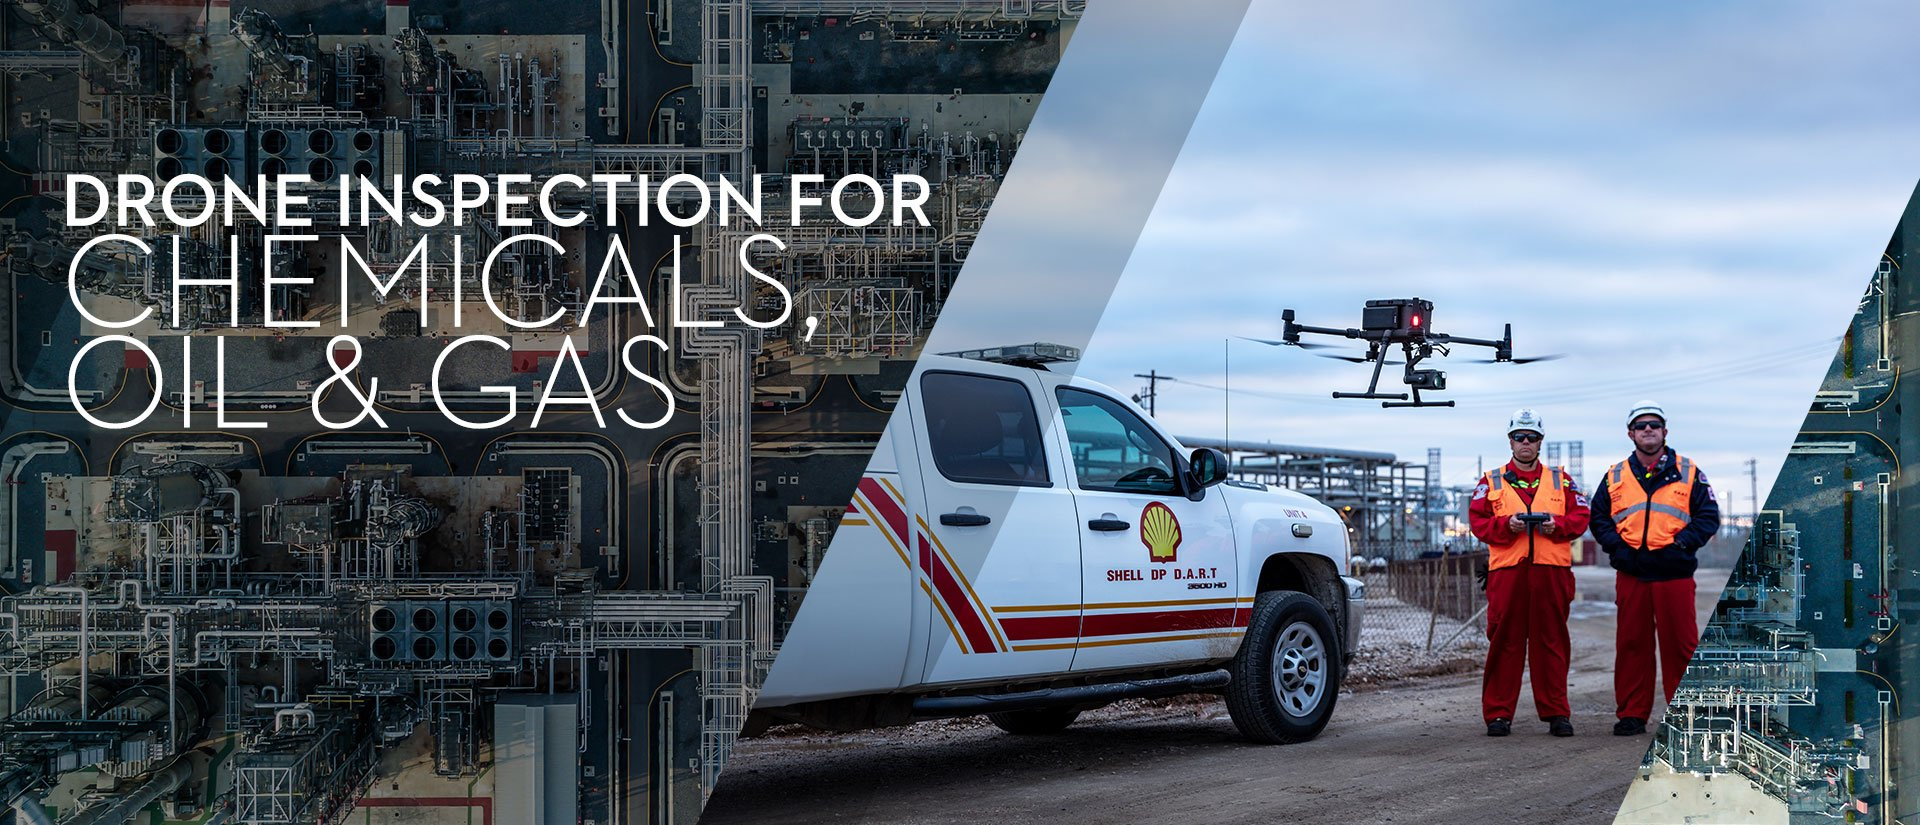
\includegraphics[width=\linewidth]{DJI_B4} % Reemplazar con la ruta a tu imagen
            %\caption{Segunda Imagen}
        \end{minipage}
        \vspace{-0.2cm} % Espacio vertical entre imágenes
        \begin{minipage}{0.48\textwidth}
            \centering
            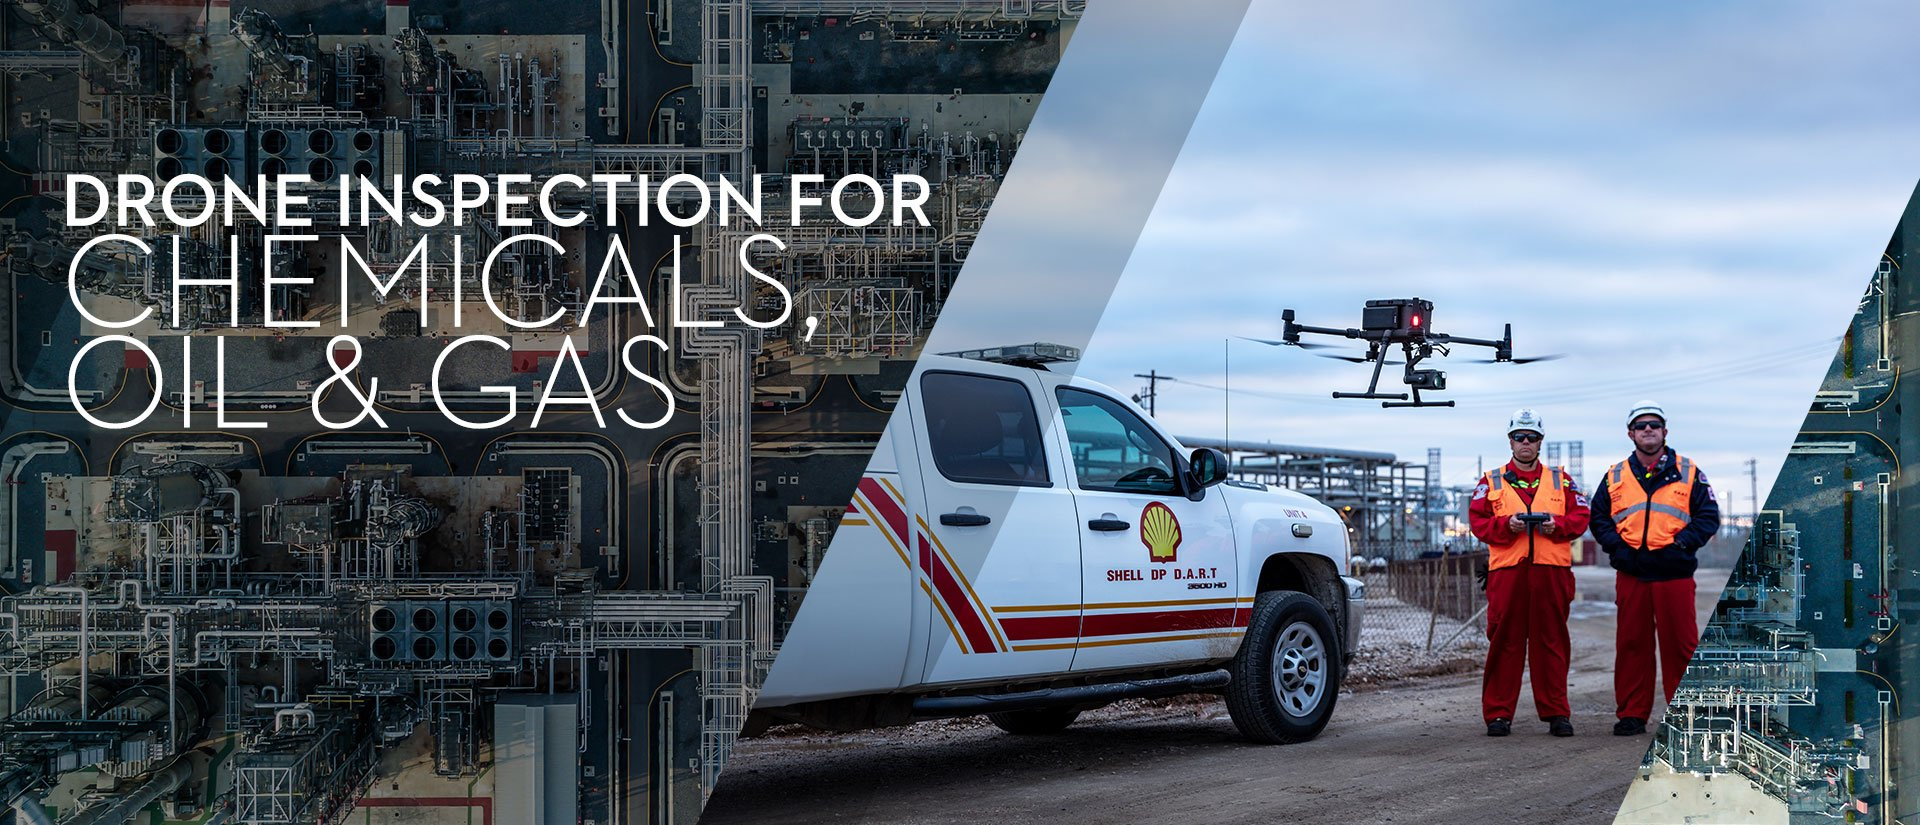
\includegraphics[width=\linewidth]{DJI_B4} % Reemplazar con la ruta a tu imagen
            %\caption{Tercera Imagen}
        \end{minipage}\hfill
        \begin{minipage}{0.48\textwidth}
            \centering
            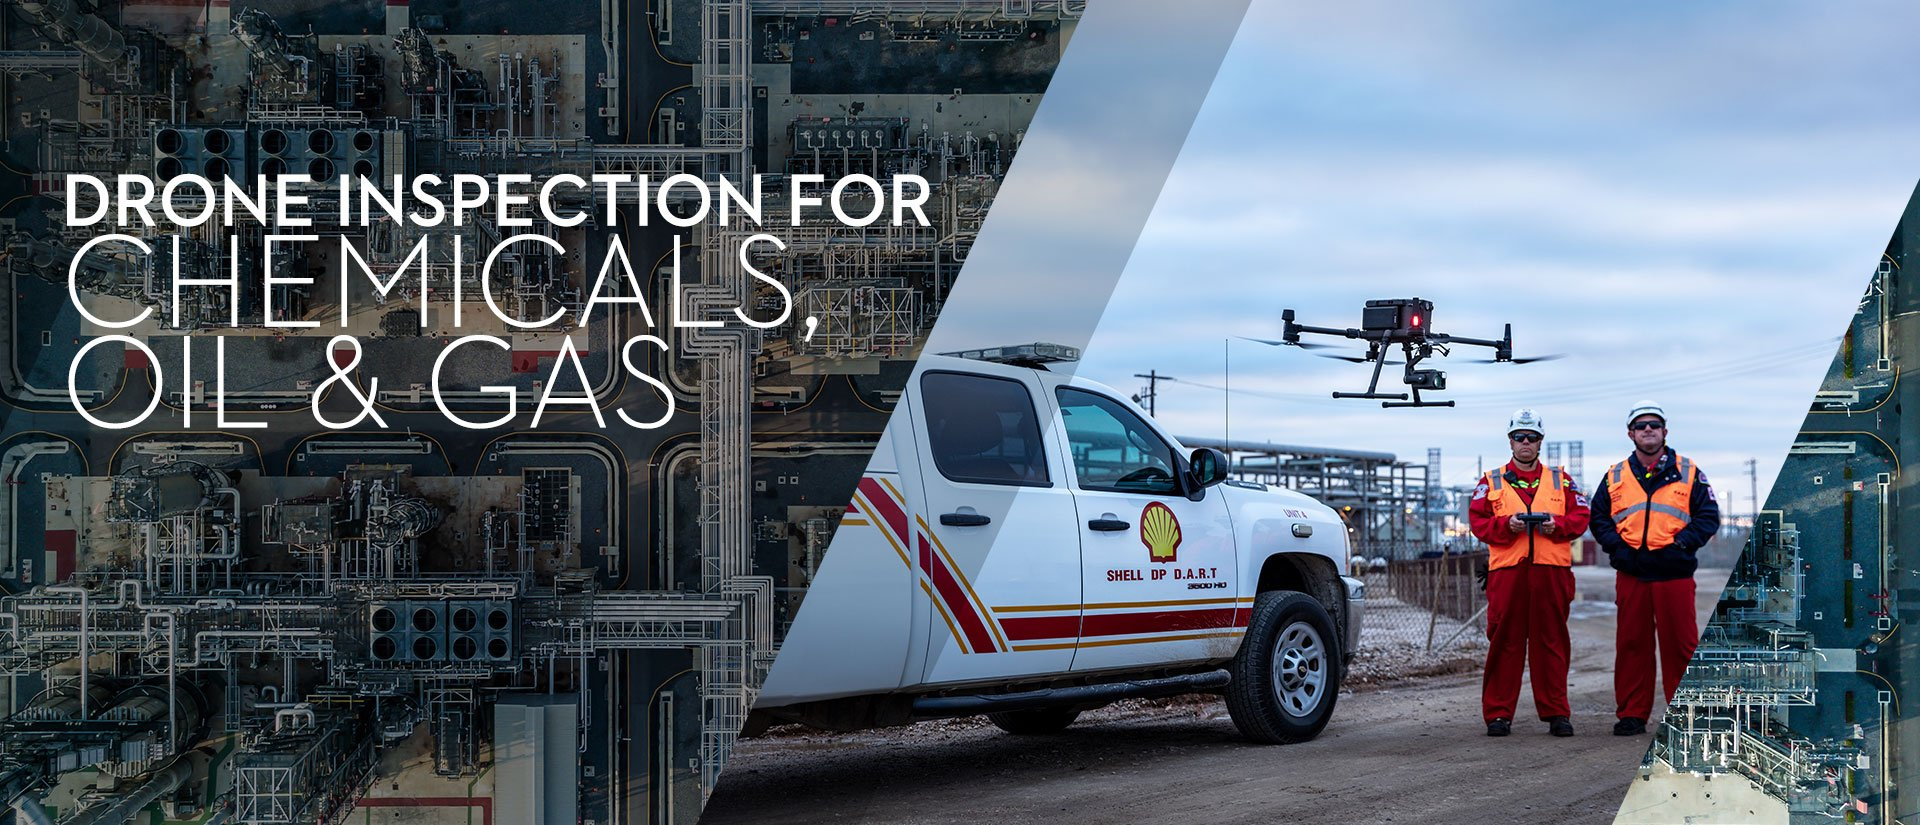
\includegraphics[width=\linewidth]{DJI_B4} % Reemplazar con la ruta a tu imagen
            %\caption{Cuarta Imagen}
        \end{minipage}
    \end{figure}
\end{frame}

\section{Planteamiento del problema}
\begin{frame}{Planteamiento del problema}
  Hacer el planteamiento del problema con los diferentes problemas:
  \begin{itemize}
  \item Dinamica del VANT
  \item SLAM VANT
  \item Exploracion
  \item Coordinacion
  \item Sistema Multi-Agente
  \end{itemize}
\end{frame}

\section{Hipótesis y preguntas de investigación}
\begin{frame}%{Hipótesis y preguntas de investigación}
  %\textbf{Exploración}\\
  %\bigskip % Vertical whitespace

  \begin{block}{Hipótesis}
    Una estrategia que coordine y asigne tareas de exploración para múltiples VANTS, en combinación con una arquitectura de software (que resuelva los problemas de localización, manejo de mapas y planificación de rutas) mejorará el desempeño en tareas de exploración con múltiples VANTS en entornos desconocidos.
  \end{block}

  Preguntas de investigación:\\
  \begin{itemize}
  \item Elección de un simulador ligero compatible con ROS.
  \item Resolver el problema de autónomia para cada agente nos aproxima a validar la hipótesis planteada.
  \item Dividir el problema en agentes individuales nos ayuda a su comprensión, y hace que el mecanismo de coordinación tome un papel importante en compañia de una función que modele las fronteras a explorar. 
  \end{itemize}
  
  %Exploración es una tarea fundamental en robots autónomos.
  %El objetivo es crear un mapa de un ambiente desconocido.\\
  %\bigskip % Vertical whitespace
  %\centering
  %
\includegraphics[width=7cm]{exploracion}\\
  
  %\begin{itemize}
  %\item \textbf{Sensar}
  %\item \textbf{Creación Mapa} 
  %\item \textbf{Localización en Mapa}
  %\item \textbf{Exploración} Aumentar la base de conocimiento del Mapa
  %\item \textbf{Planificación trayectoria} Trayectorias hacia nuevas fronteras 
  %\item \textbf{Control} Toma de decisiones y ejecución de trayectorias 
  %\end{itemize}

  %\alert{- El ciclo se repite hasta completar la exploración -}
  
\end{frame}

\section{Objetivos generales y particulares}
\begin{frame}{Objetivos generales y particulares}
  Objetivo General:\\
  \rule{0in}{1.2em}
  Objetivos Particulares:
  \begin{itemize}
  \item Obj1
  \item Obj2
  \item Obj3
  \end{itemize}
\end{frame}

\section{Estado del arte}
\begin{frame}{Estado del arte}
  Mostrar tabla
\end{frame}

\begin{frame}{Dirección estado del arte}
  Mostrar grafico de donde se encuentran los trabajos
\end{frame}

\section{Metodologia}
\begin{frame}{Metodologia}
  
  \begin{block}{Hipótesis}
    Una estrategia que coordine y asigne tareas de exploración para múltiples VANTS, en combinación con una arquitectura de software (que resuelva los problemas de localización, manejo de mapas y planificación de rutas) mejorará el desempeño en tareas de exploración con múltiples VANTS en entornos desconocidos.
  \end{block}

  \begin{itemize}
    \item Elección de un simulador ligero compatible con ROS.
    \item Resolver el problema de autónomia para cada agente nos aproxima a validar la hipótesis planteada.
    \item Dividir el problema en agentes individuales nos ayuda a su comprensión, y hace que el mecanismo de coordinación tome un papel importante en compañia de una función que modele las fronteras a explorar. 
  \end{itemize}
\end{frame}

\section{Resultados}
\begin{frame}{Resultados}
  Mostrar los avances
\end{frame}

\section{Conclusiones}
\begin{frame}{Conclusiones}
  Discusion y conclusiones
\end{frame}

\section{Cronograma de actividades}
\begin{frame}{Cronograma de actividades}
  Poner el cronograma aquí
\end{frame}

\begin{frame}[allowframebreaks,noframenumbering]{Bibliografía}
  \tiny
  \bibliographystyle{abbrvnat}
  \bibliography{test}
\end{frame}

\end{document} 
